\documentclass[8pt, xcolor={svgnames}]{beamer}
\usetheme[progressbar=frametitle]{metropolis}
\usepackage{appendixnumberbeamer}
\usepackage{url}
\usepackage{amsfonts} 
\usepackage{amssymb}
\usepackage[english]{babel}
\usepackage{fontawesome}
\usepackage{multicol}
\usepackage{bm}
\usepackage{braket}
\usepackage{algorithm}
\usepackage{algpseudocode}
\usepackage{enumitem}

\usepackage[]{pseudo}

\usepackage{tikz}
\usetikzlibrary{positioning,arrows,calc,math,angles,quotes}

\usetikzlibrary{arrows,automata}
\usetikzlibrary{positioning}
\usetikzlibrary{arrows.meta,
                bending,
                intersections,
                quotes,
                shapes.geometric}

\tikzset{
    state/.style={
           rectangle,
           rounded corners,
           draw=black, very thick,
           minimum height=1em,
           inner sep=2pt,
           text centered,
           },
}

\definecolor{cadmiumgreen}{rgb}{0.0, 0.42, 0.24}

\usepackage[most]{tcolorbox}
\usepackage{xcolor}


\title{}
\date{}
\author{}



\begin{document}

% SLIDE 1 QML
\begin{frame}{Quantum Machine Learning - doing ML using QC}

\vspace{1.5cm}

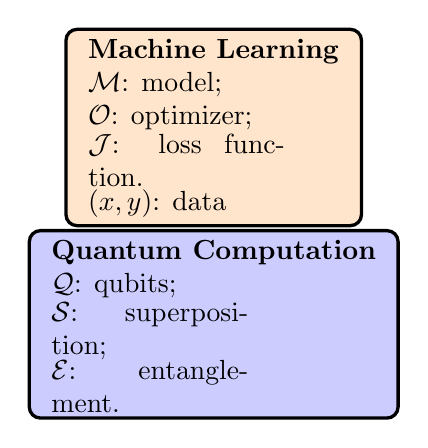
\begin{tikzpicture}[->,>=stealth']

 \node[state, fill=orange!20] (ML) 
 {\begin{tabular}{l}
 \textbf{Machine Learning}\\ 
 \parbox{2.5cm}{$\mathcal{M}$: model;}\\
 \parbox{2.5cm}{$\mathcal{O}$: optimizer;}\\
 \parbox{2.5cm}{$\mathcal{J}$: loss function.}\\
 \parbox{2.5cm}{$(x, y)$: data}
  \end{tabular}
  };
  
  \node[state,
  below of = ML,
  yshift=-1.5cm, fill=blue!20] (QC) 
 {\begin{tabular}{l}
 \textbf{Quantum Computation}\\ 
 \parbox{2.5cm}{$\mathcal{Q}$: qubits;} \\
 \parbox{2.5cm}{$\mathcal{S}$: superposition;}\\
 \parbox{2.5cm}{$\mathcal{E}$: entanglement.}
  \end{tabular}
  };
  
\end{tikzpicture}
\end{frame}


% SLIDE 2 QML
\begin{frame}{Quantum Machine Learning - operating on qubits}

\vspace{1.77cm}

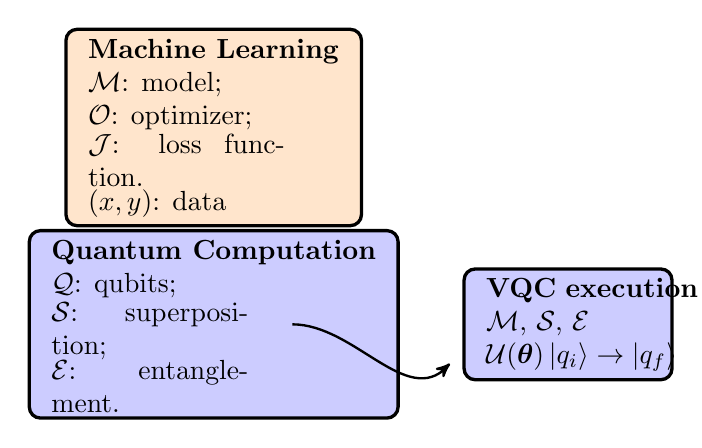
\begin{tikzpicture}[->,>=stealth']

 \node[state, fill=orange!20] (ML) 
 {\begin{tabular}{l}
 \textbf{Machine Learning}\\ 
 \parbox{2.5cm}{$\mathcal{M}$: model;}\\
 \parbox{2.5cm}{$\mathcal{O}$: optimizer;}\\
 \parbox{2.5cm}{$\mathcal{J}$: loss function.}\\
 \parbox{2.5cm}{$(x, y)$: data}
  \end{tabular}
  };
  
  \node[state,
  below of = ML,
  yshift=-1.5cm, fill=blue!20] (QC) 
 {\begin{tabular}{l}
 \textbf{Quantum Computation}\\ 
 \parbox{2.5cm}{$\mathcal{Q}$: qubits;} \\
 \parbox{2.5cm}{$\mathcal{S}$: superposition;}\\
 \parbox{2.5cm}{$\mathcal{E}$: entanglement.}
  \end{tabular}
  };
  
   \node[state,
    right of=QC,
    yshift=0cm,
    anchor=center,
    node distance=4.5cm, 	
    text width=2.5cm, fill=blue!20] (VQC) 
 {%
 \begin{tabular}{l}
  \textbf{VQC execution}\\
  $\mathcal{M}$, $\mathcal{S}$, $\mathcal{E}$ \\
  \parbox{2.8cm}{$\mathcal{U}(\bm{\theta})\ket{q_i} \to \ket{q_f}$}
 \end{tabular}
 };
 
  \draw[line width=0.3mm] (1, -2.5)  to[out=0, in=230] (3, -3);
\end{tikzpicture}

\end{frame}

% SLIDE 3 QML
\begin{frame}{Quantum Machine Learning - natural randomness}

\vspace{1.77cm}

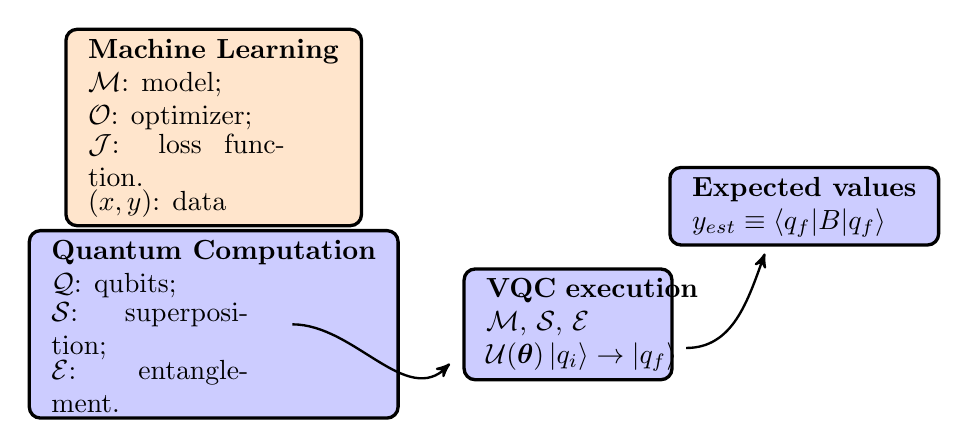
\begin{tikzpicture}[->,>=stealth']

 \node[state, fill=orange!20] (ML) 
 {\begin{tabular}{l}
 \textbf{Machine Learning}\\ 
 \parbox{2.5cm}{$\mathcal{M}$: model;}\\
 \parbox{2.5cm}{$\mathcal{O}$: optimizer;}\\
 \parbox{2.5cm}{$\mathcal{J}$: loss function.}\\
 \parbox{2.5cm}{$(x, y)$: data}
  \end{tabular}
  };
  
  \node[state,
  below of = ML,
  yshift=-1.5cm, fill=blue!20] (QC) 
 {\begin{tabular}{l}
 \textbf{Quantum Computation}\\ 
 \parbox{2.5cm}{$\mathcal{Q}$: qubits;} \\
 \parbox{2.5cm}{$\mathcal{S}$: superposition;}\\
 \parbox{2.5cm}{$\mathcal{E}$: entanglement.}
  \end{tabular}
  };
  
   \node[state,
    right of=QC,
    yshift=0cm,
    anchor=center,
    node distance=4.5cm, 	
    text width=2.5cm, fill=blue!20] (VQC) 
 {%
 \begin{tabular}{l}
  \textbf{VQC execution}\\
  $\mathcal{M}$, $\mathcal{S}$, $\mathcal{E}$ \\
  \parbox{2.8cm}{$\mathcal{U}(\bm{\theta})\ket{q_i} \to \ket{q_f}$}
 \end{tabular}
 };
 
\node[state,
  right of = VQC,
  node distance = 3cm,
  yshift=1.5cm, fill=blue!20] (NSHOT) 
 {\begin{tabular}{l}
 \textbf{Expected values}\\ 
 $y_{est} \equiv \braket{q_f|B|q_f}$
  \end{tabular}
  };
 
\draw[line width=0.3mm] (1, -2.5)  to[out=0, in=230] (3, -3);
\draw[line width=0.3mm] (6, -2.8)  to[out=0, in=250] (7, -1.6);
\end{tikzpicture}

\end{frame}


% SLIDE 4 QML
\begin{frame}{Quantum Machine Learning - encoding the problem}

\vspace{1.01cm}
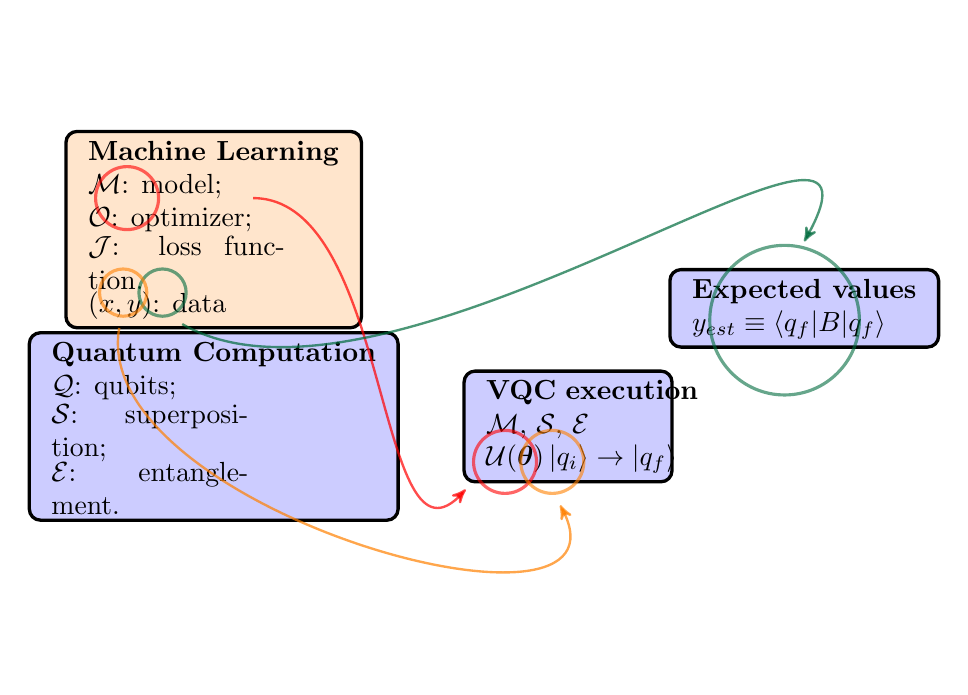
\begin{tikzpicture}[->,>=stealth']

 \node[state, fill=orange!20] (ML) 
 {\begin{tabular}{l}
 \textbf{Machine Learning}\\ 
 \parbox{2.5cm}{$\mathcal{M}$: model;}\\
 \parbox{2.5cm}{$\mathcal{O}$: optimizer;}\\
 \parbox{2.5cm}{$\mathcal{J}$: loss function.}\\
 \parbox{2.5cm}{$(x, y)$: data}
  \end{tabular}
  };
  
  \node[state,
  below of = ML,
  yshift=-1.5cm, fill=blue!20] (QC) 
 {\begin{tabular}{l}
 \textbf{Quantum Computation}\\ 
 \parbox{2.5cm}{$\mathcal{Q}$: qubits;} \\
 \parbox{2.5cm}{$\mathcal{S}$: superposition;}\\
 \parbox{2.5cm}{$\mathcal{E}$: entanglement.}
  \end{tabular}
  };
  
 
 \node[state,
    right of=QC,
    yshift=0cm,
    anchor=center,
    node distance=4.5cm, 	
    text width=2.5cm, fill=blue!20] (VQC) 
 {%
 \begin{tabular}{l}
  \textbf{VQC execution}\\
  $\mathcal{M}$, $\mathcal{S}$, $\mathcal{E}$ \\
  \parbox{2.8cm}{$\mathcal{U}(\bm{\theta})\ket{q_i} \to \ket{q_f}$}
 \end{tabular}
 };
 
\node[state,
  right of = VQC,
  node distance = 3cm,
  yshift=1.5cm, fill=blue!20] (NSHOT) 
 {\begin{tabular}{l}
 \textbf{Expected values}\\ 
 $y_{est} \equiv \braket{q_f|B|q_f}$
  \end{tabular}
  };

  
 \draw[line width=0.3mm, red, opacity = 0.7] (0.5, 0.4)  to[out=0, in=230] (3.2, -3.3);
 \draw[line width=0.3mm, orange, opacity = 0.7] (-1.2, -1.25)  to[out=260, in=300] (4.4, -3.5);
 \draw[line width=0.3mm, cadmiumgreen, opacity = 0.7] (-0.4, -1.2)  to[out=330, in=60] (7.5, -0.15);
  
 
 \draw[red, line width=0.4mm, opacity = 0.6] (3.7,-2.95) circle (0.4 cm);
 \draw[red, line width=0.4mm, opacity = 0.6] (-1.1, 0.4) circle (0.4 cm);
 \draw[cadmiumgreen, line width=0.4mm, opacity = 0.6] (-0.65,-0.8) circle (0.3 cm);
 \draw[cadmiumgreen, line width=0.4mm, opacity = 0.6] (7.25,-1.15) circle (0.95 cm);
 \draw[orange, line width=0.4mm, opacity = 0.6] (4.3,-2.95) circle (0.4 cm);
 \draw[orange, line width=0.4mm, opacity = 0.6] (-1.15,-0.8) circle (0.3 cm);


\end{tikzpicture}
\end{frame}


% SLIDE 5 QML
\begin{frame}{Quantum Machine Learning!}

\vspace{0.25cm}
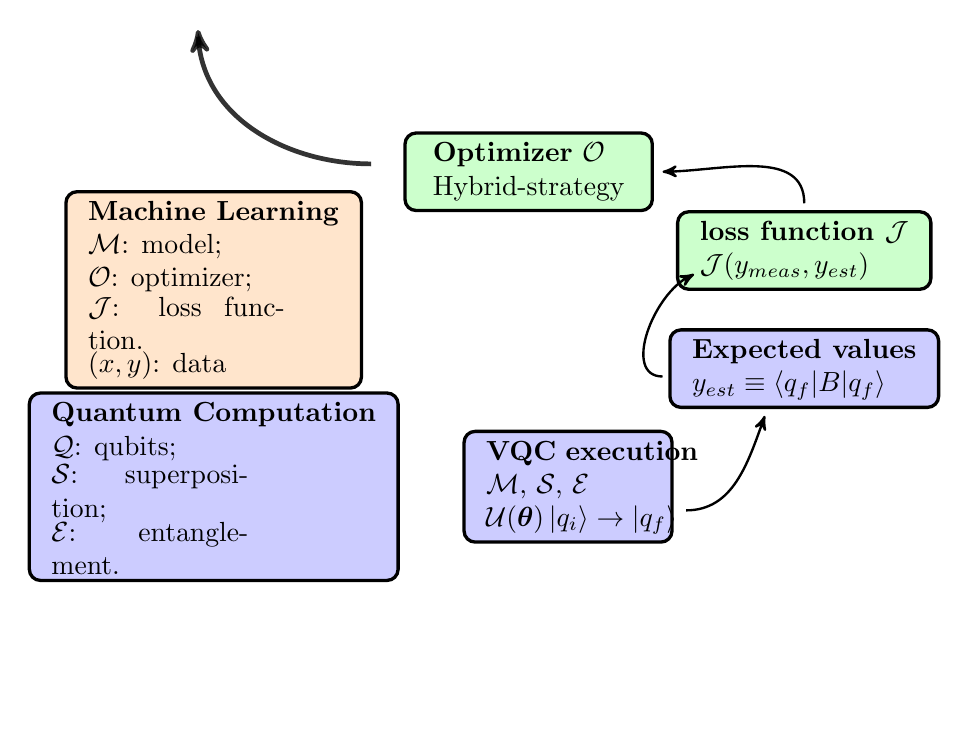
\begin{tikzpicture}[->,>=stealth']


 \node[state, fill=orange!20] (ML) 
 {\begin{tabular}{l}
 \textbf{Machine Learning}\\ 
 \parbox{2.5cm}{$\mathcal{M}$: model;}\\
 \parbox{2.5cm}{$\mathcal{O}$: optimizer;}\\
 \parbox{2.5cm}{$\mathcal{J}$: loss function.}\\
 \parbox{2.5cm}{$(x, y)$: data}
  \end{tabular}
  };
  
  \node[state,
  below of = ML,
  yshift=-1.5cm, fill=blue!20] (QC) 
 {\begin{tabular}{l}
 \textbf{Quantum Computation}\\ 
 \parbox{2.5cm}{$\mathcal{Q}$: qubits;} \\
 \parbox{2.5cm}{$\mathcal{S}$: superposition;}\\
 \parbox{2.5cm}{$\mathcal{E}$: entanglement.}
  \end{tabular}
  };
  

 \node[state,   
  text width=3cm, 
  yshift=1.5cm, 
  right of=ML, 	
  node distance=4cm, 
  anchor=center, fill=green!20] (OPT) 
 {%
 \begin{tabular}{l} 	% content
  \textbf{Optimizer $\mathcal{O}$}\\
  Hybrid-strategy
 \end{tabular}
 };
 
 \node[state,
    right of=QC,
    yshift=0cm,
    anchor=center,
    node distance=4.5cm, 	
    text width=2.5cm, fill=blue!20] (VQC) 
 {%
 \begin{tabular}{l}
  \textbf{VQC execution}\\
  $\mathcal{M}$, $\mathcal{S}$, $\mathcal{E}$ \\
  \parbox{2.8cm}{$\mathcal{U}(\bm{\theta})\ket{q_i} \to \ket{q_f}$}
 \end{tabular}
 };
 
\node[state,
  right of = VQC,
  node distance = 3cm,
  yshift=1.5cm, fill=blue!20] (NSHOT) 
 {\begin{tabular}{l}
 \textbf{Expected values}\\ 
 $y_{est} \equiv \braket{q_f|B|q_f}$
  \end{tabular}
  };
  
  \node[state,
  above of = NSHOT,
  node distance = 1.5cm,
  yshift=0cm, fill=green!20] (J) 
 {\begin{tabular}{l}
 \textbf{loss function $\mathcal{J}$}\\ 
 $\mathcal{J}(y_{meas}, y_{est})$
  \end{tabular}
  };
  

 \draw[line width=0.3mm] (6, -2.8)  to[out=0, in=250] (7, -1.6);
 \draw[line width=0.3mm] (5.7, -1.1)  to[out=180, in=200] (6.1, 0.2);
 \draw[line width=0.3mm] (7.5, 1.1)  to[out=90, in=0] (5.7, 1.5);
 \draw[line width=0.6mm, opacity=0.8] (2, 1.6)  to[out=180, in=270] (-0.2, 3.3);
 
 \draw[line width=0.3mm, orange, opacity = 0.0] (-1.2, -1.25)  to[out=260, in=300] (4.4, -3.5);

\end{tikzpicture}
\end{frame}


\begin{frame}{Density estimation with adiabatic QML  \hfill \faBook\,\, \href{https://arxiv.org/abs/2303.11346}{arXiv:2303.11346}}
\small
\faCrosshairs\,\, Determining Probability Density Functions (PDF) by fitting the 
corresponding Cumulative Density Function (CDF) using an adiabatic QML ansatz.

\faFlash\,\, Algorithm's summary:
\begin{itemize}[noitemsep]
\item[1.] we optimize the parameters $\bm{\theta}$ of the following adiabatic evolution:
\begin{equation} 
H_{\rm ad}(\tau; \bm{\theta}) = [1-s(\tau; \bm{\theta})] \hat{X} + s(\tau; \bm{\theta})\hat{Z}
\end{equation}
in order to approximate some target CDF values with $\hat{F}(x_k \equiv \tau) = \braket{\psi(\tau)|\hat{Z}|\psi(\tau)}$;
\item[2.] we derivate from $H_{\rm ad}$ a circuit $\mathcal{C}(\tau; \bm{\theta})$ whose action 
on the GS of $\hat{X}$ returns $\ket{\psi(\tau)}$;
\item[3.] the circuit at step 2. can be used to calculate the CDF;
\item[4.] we compute the PDF by derivating $\mathcal{C}$ with respect to $\tau$ 
using the Parameter Shift Rule.
\end{itemize}
\begin{figure}  
    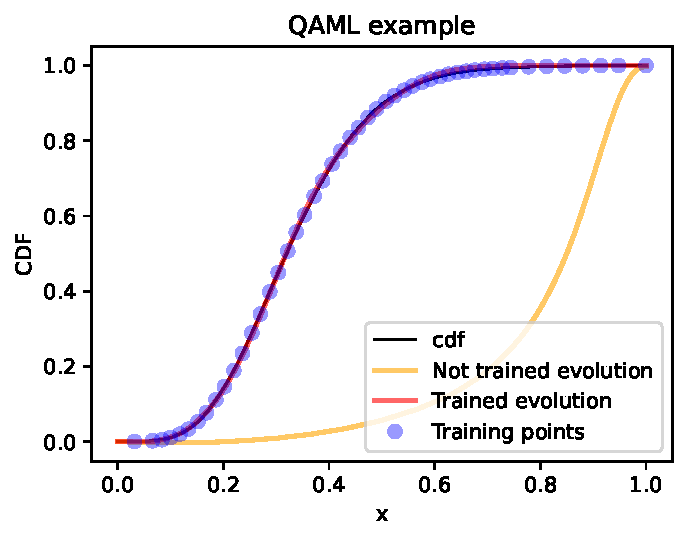
\includegraphics[width=0.5\textwidth]{figures/evolution.pdf}%
    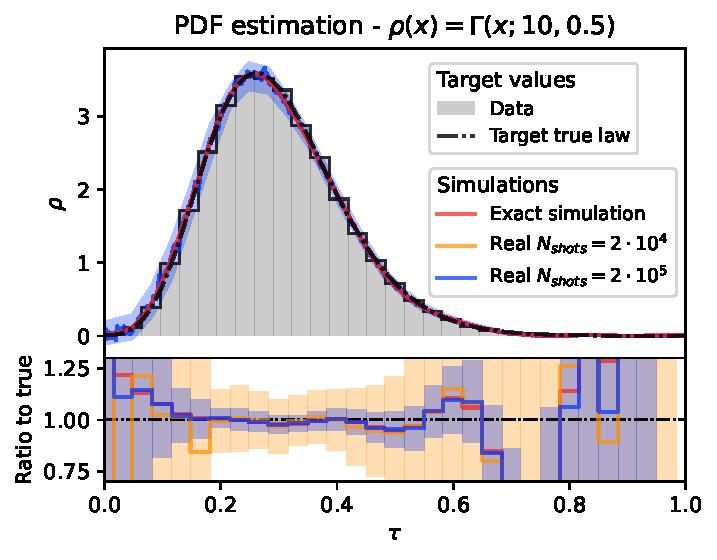
\includegraphics[width=0.5\textwidth]{figures/PDF.pdf}
\end{figure}


\end{frame}

\begin{frame}{Multi-variable integration with VQCs \hfill \faBook\,\, \href{https://arxiv.org/abs/2308.05657}{arXiv:2308.05657}}
\small
\faCrosshairs\,\, Use Variational Quantum Circuits to calculate multi-dimensional 
integrals of the form:
\begin{equation}
I(\alpha) = \int_{\bm{x}_a}^{\bm{x}_b} g(\alpha; \bm{x}) \text{d}^n \bm{x}.
\label{eq:integral}
\end{equation}

\faFlash\,\, Algorithm's summary:

\begin{itemize}[noitemsep]
\item[1.] inspired by \href{https://arxiv.org/abs/2211.02834}{arXiv:2211.02834}, 
we train the derivative of a VQC with respect to the integral variables $\bm{x}$ to approximate 
the integrand $g(\bm{x})$;
\item[2.] the derivatives are computed using the Parameter Shift Rule and this
allows the same circuit $\mathcal{C}$ to be used for approximating any integrand 
marginalisation and the primitive!
\item[3.] thanks to 2., it's much more convenient to compute Eq.~\eqref{eq:integral}
when varying $\alpha$.
\end{itemize}
\begin{figure}  
    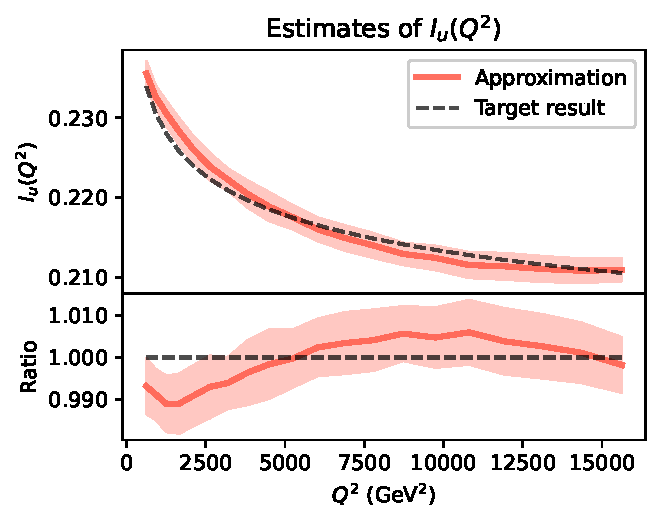
\includegraphics[width=0.5\textwidth]{figures/uquark2d.pdf}%
    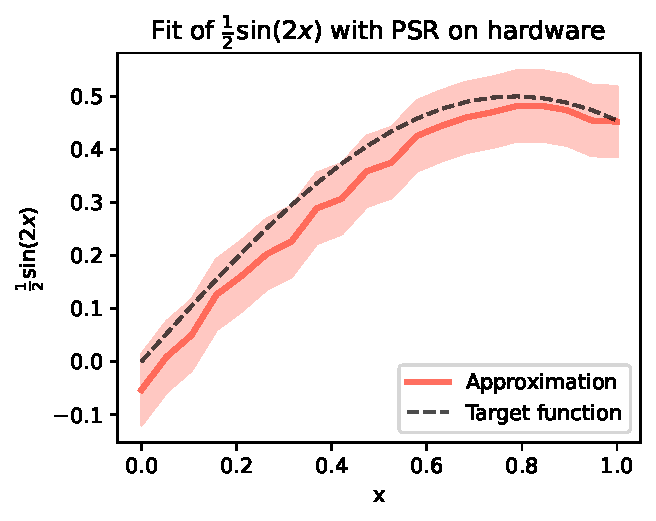
\includegraphics[width=0.5\textwidth]{figures/hardware_int.pdf}
\end{figure}
\end{frame}

\begin{frame}{Real time error mitigation in QML trainings \hfill \faBook\,\, Coming soon!}
\small
\faCrosshairs\,\, Cleaning up the parameters space with a real time error mitigation
strategy in order to overcome Noise-Induced Barren Plateaus (NIBP) when training 
a QML model.

\faFlash\,\, Algorithm's summary:

\begin{itemize}[noitemsep]
\item[1.] we mitigate all the expected values $E$ through Clifford Data Regression (CDR):
\begin{equation}
E_{\rm mit} = \alpha_{\rm cdr} E_{\rm noisy} + \beta_{\rm cdr};
\end{equation}
\item[2.] reduced CDR computational cost by updating $(\alpha, \beta)_{\rm cdr}$
periodically during the training;
\item[3.] the mitigation removes the bounds and accelerate the training process.
\end{itemize}
\begin{figure}  
    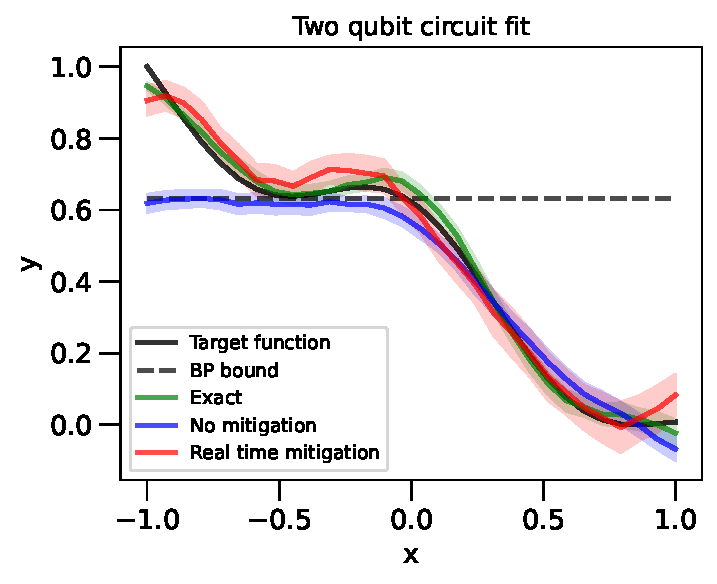
\includegraphics[width=0.5\textwidth]{figures/fits_benchmark.pdf}%
    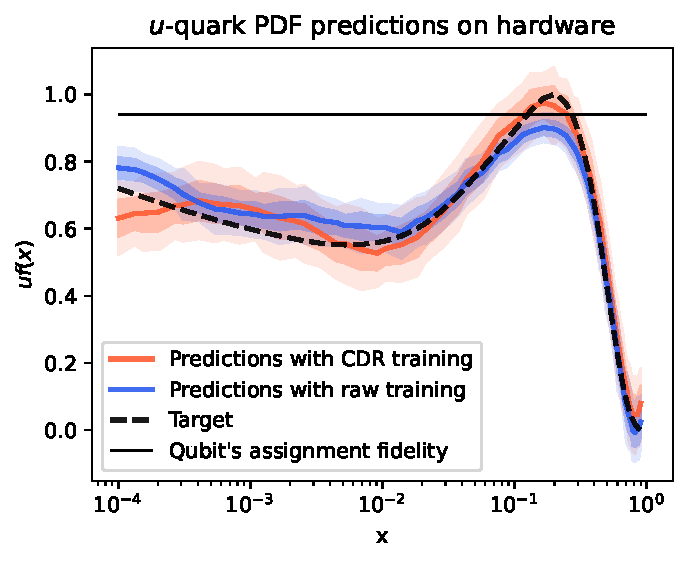
\includegraphics[width=0.5\textwidth]{figures/hardware.pdf}
\end{figure}
\end{frame}

\end{document}
